\setlength{\columnsep}{3pt}
\begin{flushleft}
Commands to display RAM related details:
\begin{itemize}
	
	\item free: Display information about the total amount of the physical \& swap memory in bytes.
	
	\begin{tcolorbox}[breakable,notitle,boxrule=-0pt,colback=pink,colframe=pink]
		\color{black}
		\fontdimen2\font=9pt
		Syntax: free
		\fontdimen2\font=4pt
	\end{tcolorbox}
	Eg:
	\begin{figure}[h!]
		\centering
		\includegraphics[scale=.3]{content/chapter12/images/free.png}
		\caption{Sample output}
		\label{fig:cpu1}
	\end{figure}
	
	Understanding the output:
	\begin{itemize}
		\item \textbf{total} - Total RAM.
		\item \textbf{used} - Used memory. It is calculated as: \textbf{used = total - free - buffers - cache}.
		\item \textbf{free} - Free / unused memory.
		\item \textbf{shared} - It has no meaning. It is here only for backward compatibility.
		\item \textbf{buff/cache} - The combined memory used by the buffers and cache. This memory can be reclaimed at any time if needed by the applications.
		\item \textbf{available} - Amount of memory available for starting new applications, without swapping.
	\end{itemize}
	\bigskip
	\begin{tcolorbox}[breakable,notitle,boxrule=-0pt,colback=yellow,colframe=yellow]
		\color{black}
		Note: You should always refer the \textbf{available} column to understand how much memory is available.
	\end{tcolorbox}
	\newpage
	
	Options with \textbf{free} command:
	\begin{itemize}
		\item \textbf{-h}: Human readable format.
		\bigskip
		\begin{tcolorbox}[breakable,notitle,boxrule=-0pt,colback=pink,colframe=pink]
			\color{black}
			\fontdimen2\font=9pt
			Syntax: free -h
			\fontdimen2\font=4pt
		\end{tcolorbox}
		Eg:
		\begin{figure}[h!]
			\centering
			\includegraphics[scale=.3]{content/chapter12/images/free_h.png}
			\caption{Sample output}
			\label{fig:free_h}
		\end{figure}

	Notice the size is displayed in \textbf{"Gi"} and not \textbf{GB}. Let's understand difference between \textbf{"Gi"} \& \textbf{"GB"}.
	
	\paragraph{UnitsPolicy}
	\begin{itemize}
		\item Base-2 units:
		\begin{itemize}
			\item 1 KiB (Kibibyte) = 1,024 bytes (Note: big k)
			\item 1 MiB (Mebibyte) = 1,024 KiB
			\item \textbf{1 GiB (Gibibyte) = 1,024 MiB}
			\item 1 TiB (Tebibyte) = 1,024 GiB
		\end{itemize}
		\bigskip
		\item Base-10 units:
		\begin{itemize}
			\item 1 kB (Kilobyte) = 1,000 bytes (Note: small k)
			\item 1 MB (Megabyte) = 1,000 kB
			\item \textbf{1 GB (Gigabyte) = 1,000 MB}
			\item 1 TB (Terabytes) = 1,000 GB
		\end{itemize}
	\end{itemize}

	To conclude,
	\bigskip
	\begin{tcolorbox}[breakable,notitle,boxrule=-0pt,colback=pink,colframe=pink]
		\color{black}
		\fontdimen2\font=9pt
		\begin{itemize}
			\item 1 GB = 0.93 GiB
			\item 1 GiB = 1.07 GB
			\item This is approx 7\% difference and can make huge difference.
		\end{itemize}	
		\fontdimen2\font=4pt
	\end{tcolorbox}

	\newpage
	\item \textbf{-w}: Display buffer and cache separately.
	\bigskip
	\begin{tcolorbox}[breakable,notitle,boxrule=-0pt,colback=pink,colframe=pink]
		\color{black}
		\fontdimen2\font=9pt
		Syntax: free -w
		\fontdimen2\font=4pt
	\end{tcolorbox}
	Eg:
	\begin{figure}[h!]
		\centering
		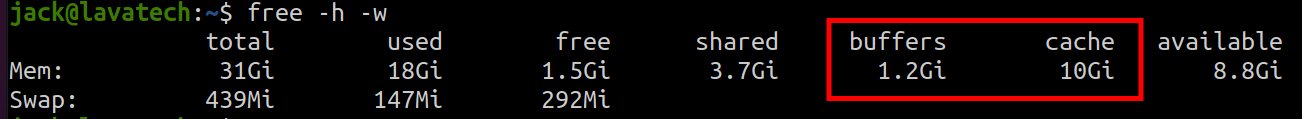
\includegraphics[scale=.25]{content/chapter12/images/free_3.png}
		\caption{Sample output}
		\label{fig:free_3}
	\end{figure}

\bigskip
\bigskip
	
	\end{itemize}
	
	\item Display top 10 processes consuming highest amount of RAM:
	\bigskip
	\begin{tcolorbox}[breakable,notitle,boxrule=-0pt,colback=pink,colframe=pink]
		\color{black}
		\fontdimen2\font=9pt
		Syntax: ps -eo pid,ppid,cmd,\%mem,\%cpu --sort=-\%mem | head
		\fontdimen2\font=4pt
	\end{tcolorbox}
	Eg:
	\begin{figure}[h!]
		\centering
		\includegraphics[scale=.3]{content/chapter12/images/ps_1.png}
		\caption{Sample output}
		\label{fig:ps_1}
	\end{figure}
	\newpage
	\item Command to sort all process with maximum memory consumption:
		\bigskip
	\begin{tcolorbox}[breakable,notitle,boxrule=-0pt,colback=pink,colframe=pink]
		\color{black}
		\fontdimen2\font=9pt
		Syntax: top
		\newline
		\color{blue}
		Press "M" to sort task list by processor usage
		\fontdimen2\font=4pt
	\end{tcolorbox}
	Eg:
	\begin{figure}[h!]
		\centering
		\includegraphics[scale=.4]{content/chapter12/images/mem.png}
		\caption{Sample output}
		\label{fig:cpu25}
	\end{figure}
	
	
\end{itemize}

	\textbf{When should I start to worry about my RAM?}
	\bigskip
	\begin{itemize}
		\item Below values in \textbf{free} command shows \color{blue} \textbf{healthy Linux system}\color{black}:
		\begin{itemize}
			\item \textbf{Free memory} is close to \textbf{0}.
			\item \textbf{Used memory} is close to \textbf{total}.
			\item \textbf{Available memory} should have approx. \textbf{20\%+ of total}.
			\item Swap used does not change.
		\end{itemize}
		\bigskip
		\item  Below values are \color{red} \textbf{warning signs} \color{black} of a genuine low memory situation:
		\begin{itemize}
			\item \textbf{Available memory} is close to \textbf{zero}.
			\item \textbf{Swap} used \textbf{increases or fluctuates}.
			\item Command "dmesg | grep oom-killer" shows the \textbf{OutOfMemory-killer} at work.
		\end{itemize}
	\end{itemize}
	
	
\end{flushleft}

\newpage


